    \documentclass[tikz, border=10pt]{standalone}
    \usepackage{amsmath}
    \usepackage{amssymb}
    \usetikzlibrary{positioning, arrows.meta, backgrounds, calc, shapes.geometric, decorations.pathreplacing}

    % ==========================================
    % 高级柔和配色 (与原网络结构图完全一致)
    % ==========================================
    \definecolor{b1fill}{RGB}{235, 245, 255}
    \definecolor{b1draw}{RGB}{21, 101, 192}   % 蓝色系 (Train / Input)

    \definecolor{b2fill}{RGB}{249, 251, 235}
    \definecolor{b2draw}{RGB}{130, 119, 23}   % 绿黄色系 (Val / Sliding)

    \definecolor{b3fill}{RGB}{255, 240, 240}
    \definecolor{b3draw}{RGB}{192, 57, 43}    % 红色系 (Test / Output)

    \definecolor{opfill}{RGB}{245, 247, 250}
    \definecolor{opdraw}{RGB}{84, 110, 122}   % 灰色系 (Tensor)

    \begin{document}
    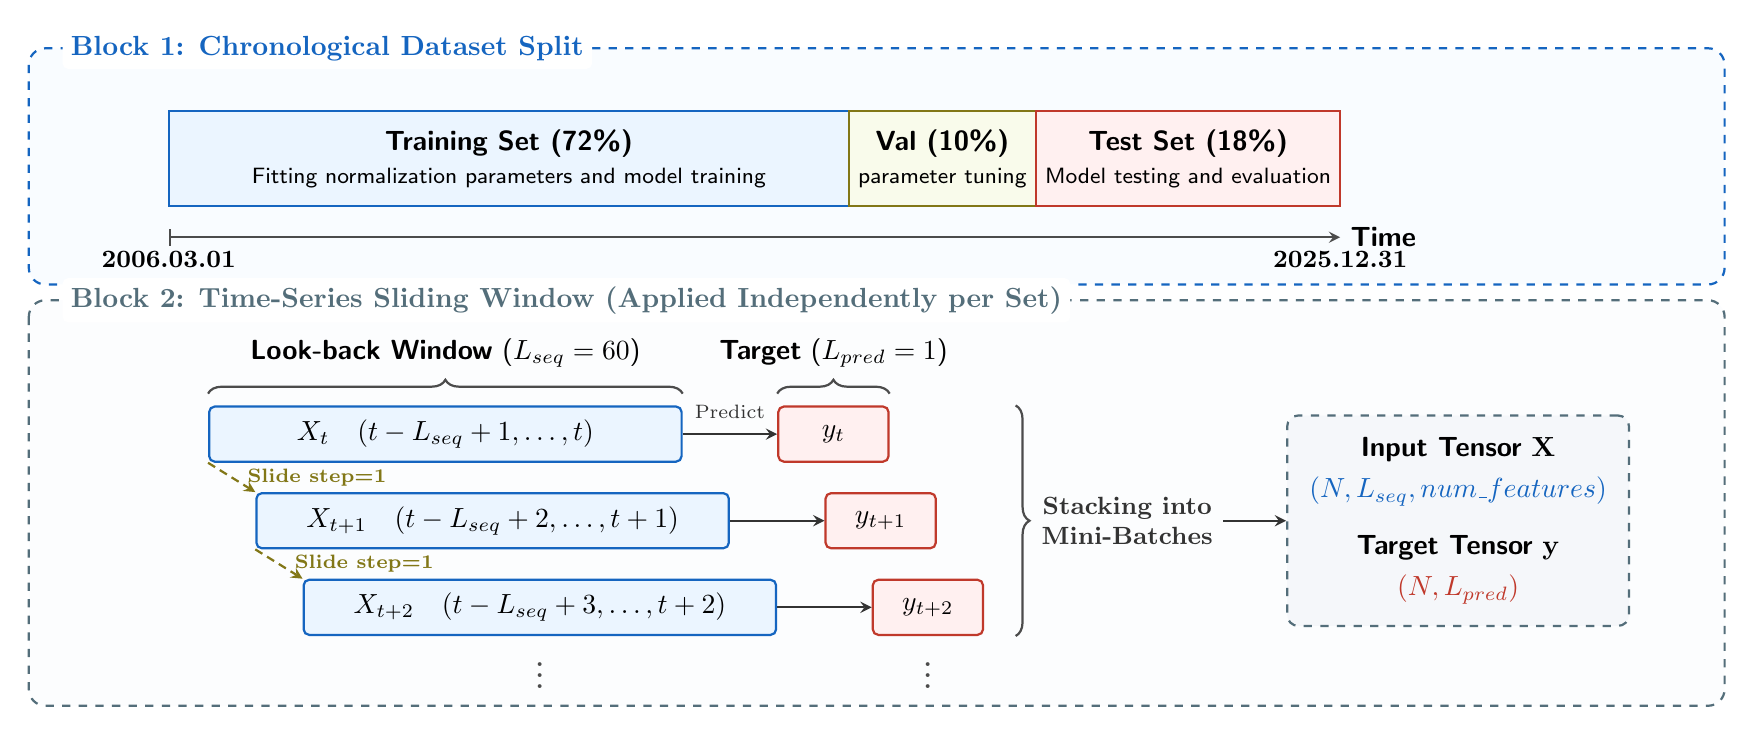
\begin{tikzpicture}[
        >=stealth,
        font=\sffamily,
        % 数据集划分框样式
        trainbox/.style={draw=b1draw, fill=b1fill, thick, minimum height=1.2cm, align=center, outer sep=0pt},
        valbox/.style={draw=b2draw, fill=b2fill, thick, minimum height=1.2cm, align=center, outer sep=0pt},
        testbox/.style={draw=b3draw, fill=b3fill, thick, minimum height=1.2cm, align=center, outer sep=0pt},
        % 滑动窗口特征与标签样式
        seqbox/.style={draw=b1draw, fill=b1fill, thick, rounded corners=2pt, minimum height=0.7cm, align=center},
        labelbox/.style={draw=b3draw, fill=b3fill, thick, rounded corners=2pt, minimum height=0.7cm, minimum width=1.4cm, align=center},
        tensorbox/.style={draw=opdraw, fill=opfill, dashed, thick, rounded corners=4pt, align=center, inner sep=8pt},
        % 背景大框样式
        groupbox/.style={draw=#1draw, thick, dashed, rounded corners=6pt, fill=#1fill!30},
        % 连线与辅助样式
        arrow/.style={->, thick, draw=black!80, rounded corners=4pt},
        brace/.style={decorate, decoration={brace, amplitude=5pt}, thick, draw=black!70}
    ]

    % ==========================================
    % 1. 上半部分：数据集按时间顺序划分 (Macro Level)
    % ==========================================
    % 以精确比例绘制宽度：总宽度约为 12cm，72% -> 8.64cm, 10% -> 1.2cm, 18% -> 2.16cm
    \node[trainbox, minimum width=8.64cm, anchor=west] (train) at (0, 0) {\textbf{Training Set (72\%)}\\ \footnotesize Fitting normalization parameters and model training};
    \node[valbox, minimum width=1.2cm, anchor=west] (val) at (train.east) {\textbf{Val (10\%)}\\\footnotesize parameter tuning};
    \node[testbox, minimum width=2.16cm, anchor=west] (test) at (val.east) {\textbf{Test Set (18\%)}\\\footnotesize Model testing and evaluation};

    % 时间轴 (增加底部 padding 避免文字太挤)
    \draw[|->, thick, draw=black!70] ($(train.south west) + (0, -0.4)$) -- ($(test.south east) + (0, -0.4)$) node[right] {\textbf{Time}};

    % 为时间节点命名，方便后面计算边界框（修复问题1）
    \node[below=0.45cm of train.south west, anchor=north, font=\small\bfseries] (date_start) {2006.03.01};
    \node[below=0.45cm of test.south east, anchor=north, font=\small\bfseries] (date_end) {2025.12.31};

    % (修复问题5：去除了两条多余的虚线)

    % ==========================================
    % 2. 下半部分：时序滑动窗口切分 (Micro Level)
    % ==========================================
    \coordinate (zoom_center) at (0.5, -3.5);

    % --- 第一个窗口 (t) ---
    \node[seqbox, minimum width=6cm, anchor=west] (x1) at ($(zoom_center) + (0, 0)$) {$X_t \quad (t-L_{seq}+1, \dots, t)$};
    % (修复问题2：增加了 X 和 y 之间的水平间距到 1.2cm，避免箭头和文字拥挤)
    \node[labelbox, anchor=west] (y1) at ($(x1.east) + (1.2cm, 0)$) {$y_t$};
    % 增加 above=2pt 抬高文字，避免覆盖线条
    \draw[arrow] (x1) -- node[above=2pt, font=\scriptsize, color=black!80] {Predict} (y1);

    % 顶部大括号标注
    \draw[brace] ($(x1.north west) + (0, 0.15)$) -- ($(x1.north east) + (0, 0.15)$) node[midway, above=0.2cm] {\textbf{Look-back Window} ($L_{seq}=60$)};
    \draw[brace] ($(y1.north west) + (0, 0.15)$) -- ($(y1.north east) + (0, 0.15)$) node[midway, above=0.2cm] {\textbf{Target} ($L_{pred}=1$)};

    % --- 第二个窗口 (t+1) ---
    \node[seqbox, minimum width=6cm, anchor=west] (x2) at ($(zoom_center) + (0.6, -1.1)$) {$X_{t+1} \quad (t-L_{seq}+2, \dots, t+1)$};
    \node[labelbox, anchor=west] (y2) at ($(x2.east) + (1.2cm, 0)$) {$y_{t+1}$};
    \draw[arrow] (x2) -- (y2);

    % --- 第三个窗口 (t+2) ---
    \node[seqbox, minimum width=6cm, anchor=west] (x3) at ($(zoom_center) + (1.2, -2.2)$) {$X_{t+2} \quad (t-L_{seq}+3, \dots, t+2)$};
    \node[labelbox, anchor=west] (y3) at ($(x3.east) + (1.2cm, 0)$) {$y_{t+2}$};
    \draw[arrow] (x3) -- (y3);

    % 省略号 (修复问题6：动态锚定到 x3 和 y3 的底部中心，保证绝对居中)
    \node[font=\Large, color=black!70] at ($(x3.south) + (0, -0.4)$) {$\vdots$};
    \node[font=\Large, color=black!70] at ($(y3.south) + (0, -0.4)$) {$\vdots$};

    % 滑动步长标注 (稍微往右移一点点(0.5)会更协调)
    \draw[arrow, b2draw, densely dashed] ($(x1.south west) + (0, 0)$) -- node[right=2pt, font=\scriptsize, color=b2draw] {\textbf{Slide step=1}} ($(x2.north west) + (0, 0)$);
    \draw[arrow, b2draw, densely dashed] ($(x2.south west) + (0, 0)$) -- node[right=2pt, font=\scriptsize, color=b2draw] {\textbf{Slide step=1}} ($(x3.north west) + (0, 0)$);


    % ==========================================
    % 3. 右侧：张量合并堆叠
    % ==========================================
    % (修复问题4：强制大括号绝对竖直！取 y3 的东面作为统一 X 坐标)
    \coordinate (brace_top) at ($(y3.east |- y1.north) + (0.4cm, 0)$);
    \coordinate (brace_bot) at ($(y3.east |- y3.south) + (0.4cm, 0)$);

    % (修复问题3：添加 right=0.2cm padding 解决字压线问题)
    \draw[brace] (brace_top) -- (brace_bot) node[midway, right=0.2cm, align=center, font=\small\bfseries, color=black!80] (stack_text) {Stacking into\\Mini-Batches};

    % 将张量框直接相对 stack_text 定位，确保无论文字多长都不会发生重叠
    \node[tensorbox, right=0.8cm of stack_text] (tensor) {
        \textbf{Input Tensor} $\mathbf{X}$ \\[0.1cm]
        \textcolor{b1draw}{$(N, L_{seq}, num\_features)$} \\[0.3cm]
        \textbf{Target Tensor} $\mathbf{y}$ \\[0.1cm]
        \textcolor{b3draw}{$(N, L_{pred})$}
    };

    % 箭头从文字精准指向张量
    \draw[arrow] (stack_text) -- (tensor);


    % ==========================================
    % 4. 绘制背景区域 (背景框体系)
    % ==========================================
    \begin{scope}[on background layer]
        % Block 1 垂直边界
        \coordinate (B1_top) at ($(train.north) + (0, 0.8cm)$);
        \coordinate (B1_bot) at ($(train.south) + (0, -1.0cm)$);
        
        % (修复问题1：背景框宽度自适应计算)
        % 左边界：对齐到日期最左侧再偏移-0.8cm，确保完全包裹 2006.03.01
        % 右边界：对齐到张量框最右侧再偏移+1.2cm，确保上下两大框完美对齐且完全包裹
        \coordinate (B1_NW) at ($(date_start.west |- B1_top) + (-0.8cm, 0)$);
        \coordinate (B1_SE) at ($(tensor.east |- B1_bot) + (1.2cm, 0)$);
        \filldraw[groupbox=b1] (B1_NW) rectangle (B1_SE);

        % Block 2 垂直边界
        \coordinate (B2_top) at ($(B1_bot) + (0, -0.2cm)$);
        \coordinate (B2_bot) at ($(tensor.south) + (0, -1.0cm)$);
        \coordinate (B2_NW) at ($(B1_NW |- B2_top)$);
        \coordinate (B2_SE) at ($(B1_SE |- B2_bot)$);
        \filldraw[groupbox=op] (B2_NW) rectangle (B2_SE);
    \end{scope}

    % ==========================================
    % 5. 绘制框体标签
    % ==========================================
    \node[fill=white, font=\bfseries\color{b1draw}, right=12pt, rounded corners=2pt, inner sep=3pt] 
        at (B1_NW) {Block 1: Chronological Dataset Split};

    \node[fill=white, font=\bfseries\color{opdraw}, right=12pt, rounded corners=2pt, inner sep=3pt] 
        at (B2_NW) {Block 2: Time-Series Sliding Window (Applied Independently per Set)};

    \end{tikzpicture}
    \end{document}